\documentclass[../Article_Model_Parameters.tex]{subfiles}
\graphicspath{{\subfix{../Figures/}}}
\begin{document}
	
	Over the years, the extraction of natural substances from solid materials and liquids using solvents has been a topic of significant interest for research and development. Supercritical fluids are particularly useful in extraction processes due to their pressure-dependent dissolving power and ability to exhibit both gas- and liquid-like properties, such as fluid-like density and gas-like diffusivity. Of the various supercritical fluids available, supercritical $CO_2$ is particularly attractive due to its nontoxic, non-flammable, and non-corrosive properties. Moreover, the critical point of $CO_2$ is relatively low ($73.8$ bar and $31 ^\circ C$) compared to other fluids, making it an excellent alternative to traditional extraction techniques.
	
	Different mathematical models have been proposed to describe the extraction of valuable compounds from a fixed biomass bed, as reviewed by \citet{Huang2012}. However, the selection of an appropriate extraction model should be based on the knowledge of the physical phenomena taking place in the operational unit. Each model has its own set of assumptions and describes different mass transfer mechanisms and equilibrium relationships.
	
	Based on an analogy to heat transfer, \citet{Reverchon1993} proposed a hot ball model to describe an extraction process from solid particles containing small quantities of solute, where solubility is not a limiting factor. \citet{Sovova1994} presented the Broken-and-Intact Cell model, which describes a system where the outer surfaces of particles have been mechanically interrupted, allowing easy access of solvent to the solute from the broken cells. In contrast, the solute from the intact cells is less accessible due to high mass transfer resistance.
	
	\citet{Reverchon1996} developed a model for fluid-solid extraction, where the oil is treated as a single component, and the extraction process is controlled by internal mass transfer resistance, neglecting external mass transfer. This model, however, does not consider the influence of axial dispersion or changes in density and flow rate along the bed. Our work assumes that the extraction process operates semi-continuously in a cylindrical vessel. The solvent is first brought to supercritical conditions, pumped through a fixed bed of finely chopped biomass, and the solute is extracted from the biomass. The solvent and solute are then separated in a flush drum, and the extract is collected. The feed flow rate ($F_{in}$) and inlet temperature ($T_{in}$) of the extractor can be measured and manipulated. In contrast, the vessel pressure ($P$) can be measured and manipulated, but the outlet temperature ($T_{out}$) can only be measured. Figure \ref{fig: SFE_drawing} depicts a simplified flow diagram.
	
	\begin{figure}[h!]
		\centering
		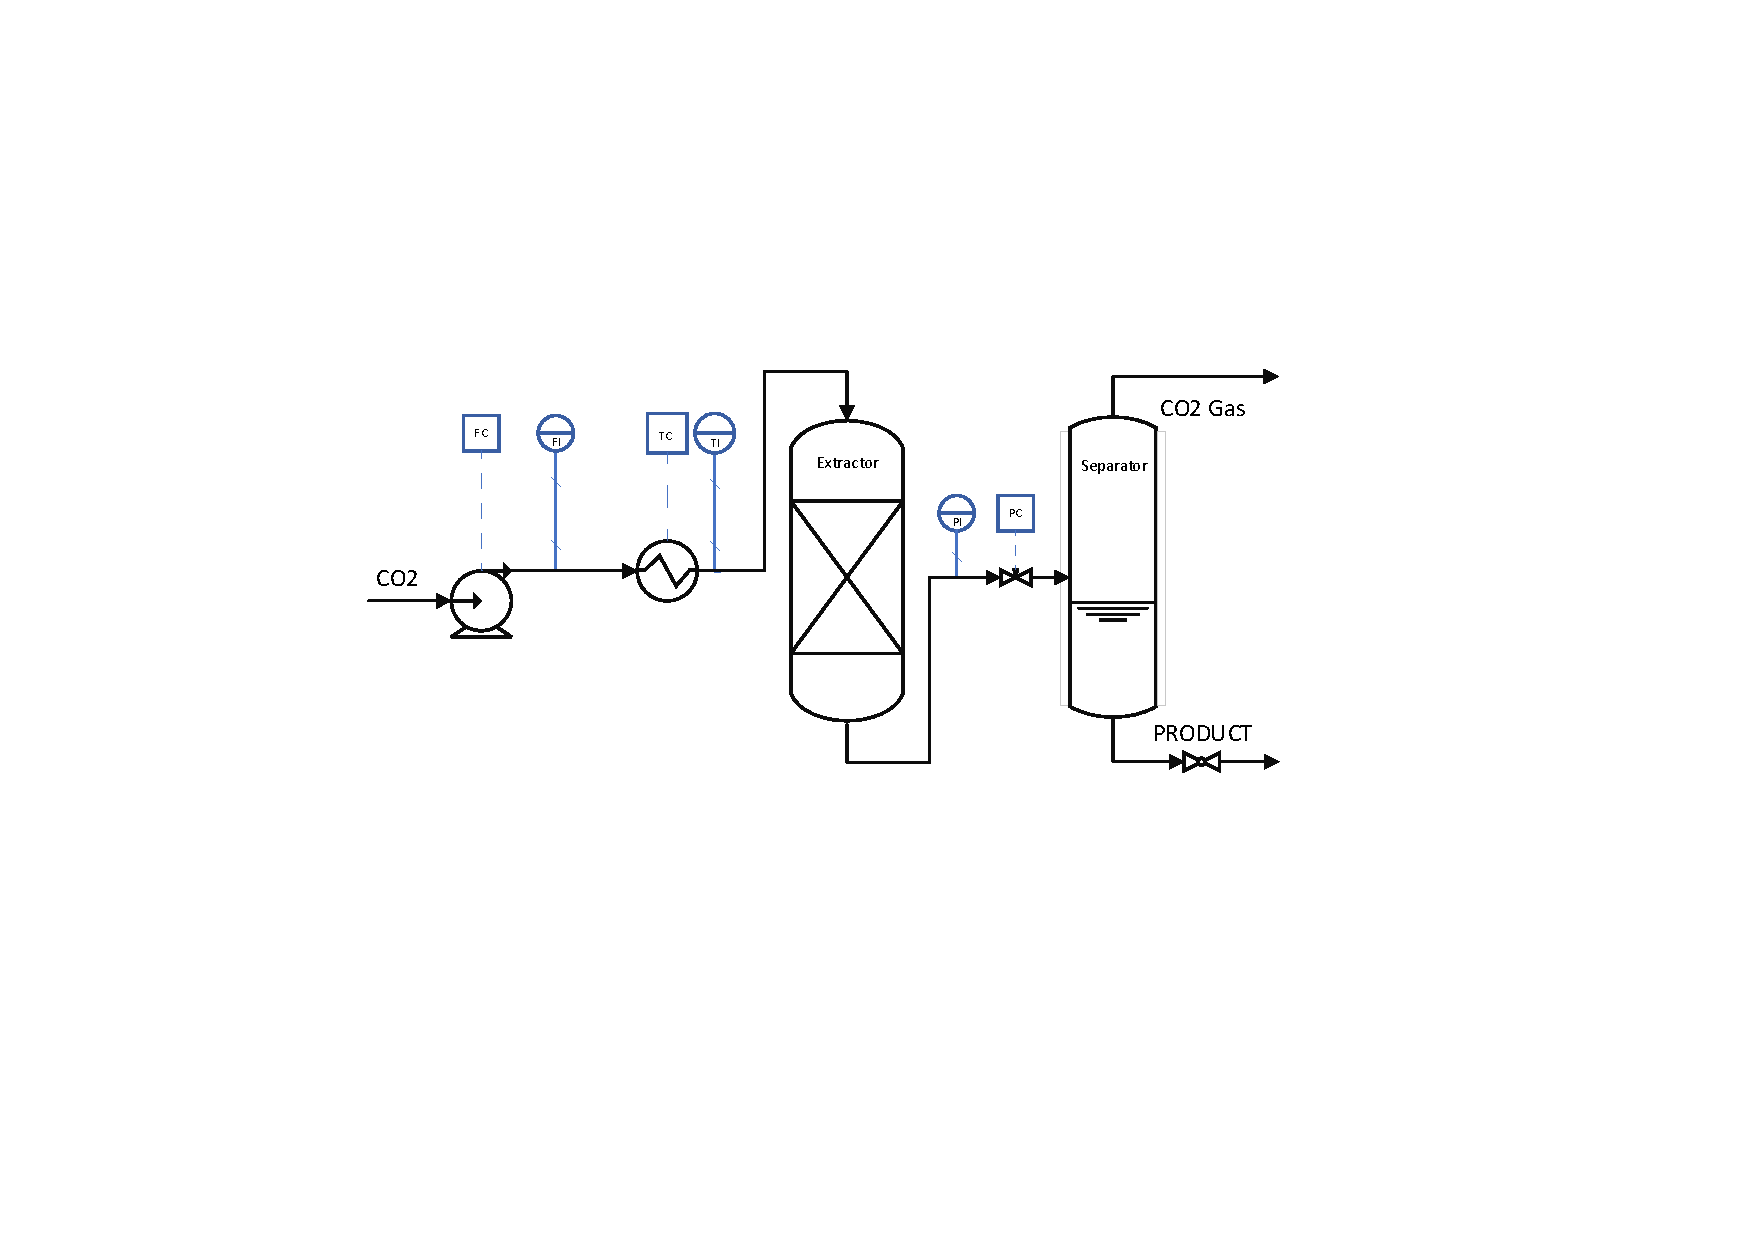
\includegraphics[width=0.95\columnwidth]{Figures/SFE_PFD_cropped.pdf}
		\caption{Process flow diagram ({\color{red}Font size}) }
		\label{fig: SFE_drawing}
	\end{figure}
	
\end{document}